\documentclass[10pt,a4paper]{article}
\usepackage[utf8]{inputenc}
\usepackage[T1]{fontenc}
\usepackage[italian]{babel}
\usepackage{lmodern}
\usepackage[margin=2.2cm]{geometry}
\usepackage{amsmath,amssymb}
\usepackage{graphicx}
\usepackage{booktabs}
\usepackage{tabularx}
\usepackage{xcolor}
\usepackage{tikz}
\usetikzlibrary{arrows.meta,positioning,fit,backgrounds}
\usepackage[hidelinks]{hyperref}
\usepackage{caption}
\captionsetup{font=small,labelfont=bf}
\graphicspath{{figs/}}

\newcommand{\WER}{\mathrm{WER}}
\definecolor{bl}{HTML}{2a6f97}
\definecolor{or}{HTML}{e07a5f}
\definecolor{gr}{HTML}{3d9970}
\definecolor{vi}{HTML}{8e6c8a}

\title{Decodificare il linguaggio dall'attività corticale:\\
una pipeline di machine learning per il Brain-to-Text Benchmark~'24}
\author{Alessandro Saccoia\\\small Università degli Studi di Milano\\\small\textit{Bozza di lavoro, \today}}
\date{}

\begin{document}
\maketitle

\begin{abstract}
Questo documento descrive il sistema in sviluppo per il \emph{Brain-to-Text Benchmark '24}, una gara pubblica (EvalAI, sfida 2099) che chiede di trascrivere in testo le frasi che una persona con paralisi tenta di pronunciare, a partire dall'attività di 256 microelettrodi impiantati nella corteccia motoria del linguaggio. Il problema è una trascrizione sequenza-a-sequenza con pochi dati (circa 10\,000 frasi di un solo partecipante) e un forte segnale non stazionario tra giorni di registrazione. La pipeline segue la struttura di un riconoscitore vocale ibrido: un decoder neurale (GRU o Transformer) addestrato con la loss CTC stima le probabilità dei fonemi, un trasduttore a stati finiti con un modello linguistico 5-gram produce le frasi candidate, e un modello linguistico di grandi dimensioni (LLM) le riordina. Il passo finale previsto è un ensemble di molti decoder fuso da un LLM addestrato. Riportiamo l'architettura, le scelte di addestramento, i primi risultati e il piano per scendere sotto il 3\% di word error rate, la soglia del primo classificato.
\end{abstract}

\section{Il problema}

Le interfacce cervello-computer per il linguaggio (\emph{speech BCI}) mirano a restituire la comunicazione a persone che hanno perso la capacità di parlare, per esempio per SLA o ictus del tronco encefalico. Willett et al.\ (\emph{Nature}, 2023) hanno mostrato che un decoder addestrato sull'attività della corteccia premotoria ventrale (area 6v) e dell'area 44 può trascrivere il parlato tentato a 62 parole al minuto con il 23\% di errore. La gara chiede di migliorare quell'algoritmo su dati pubblici e con una metrica comune.

\paragraph{Metrica.} Le predizioni sono valutate con il \emph{word error rate} su 1200 frasi di cui non si conosce la trascrizione:
\begin{equation}
\WER = \frac{\sum_{i} \mathrm{ED}(\hat w_i, w_i)}{\sum_i |w_i|},
\end{equation}
dove $\mathrm{ED}$ è la distanza di edit fra sequenze di parole (sostituzioni, inserzioni e cancellazioni) e $|w_i|$ è il numero di parole della frase di riferimento. Si possono inviare al massimo cinque sottomissioni al giorno e la gara chiude il 13 gennaio 2027. Al 22 novembre 2026 il primo classificato ha $\WER=2{,}99\%$ e la baseline ufficiale (RNN + 5-gram + OPT) il 9{,}76\%.

\section{I dati}

Il partecipante T12 aveva quattro array Utah da 64 elettrodi: due nell'area 6v e due nell'area 44. Per ogni frase il dataset fornisce, in intervalli (\emph{bin}) da 20\,ms:
\begin{itemize}\setlength\itemsep{0pt}
\item \textbf{threshold crossings} \texttt{tx1}--\texttt{tx4}: il numero di attraversamenti di soglia per canale, a quattro soglie diverse;
\item \textbf{spike-band power}: la potenza media del segnale filtrato passa-alto.
\end{itemize}
Ogni frase corrisponde quindi a una matrice $X\in\mathbb{R}^{T\times 1280}$, con $T$ fra circa 100 e 1000 bin. Seguendo la baseline usiamo \texttt{tx1} e la spike-band power dei 128 canali dell'area 6v, cioè 256 feature, che normalizziamo con uno z-score per blocco di registrazione per compensare le derive lente dei segnali (Fig.~\ref{fig:neural}).

\begin{figure}[t]
\centering
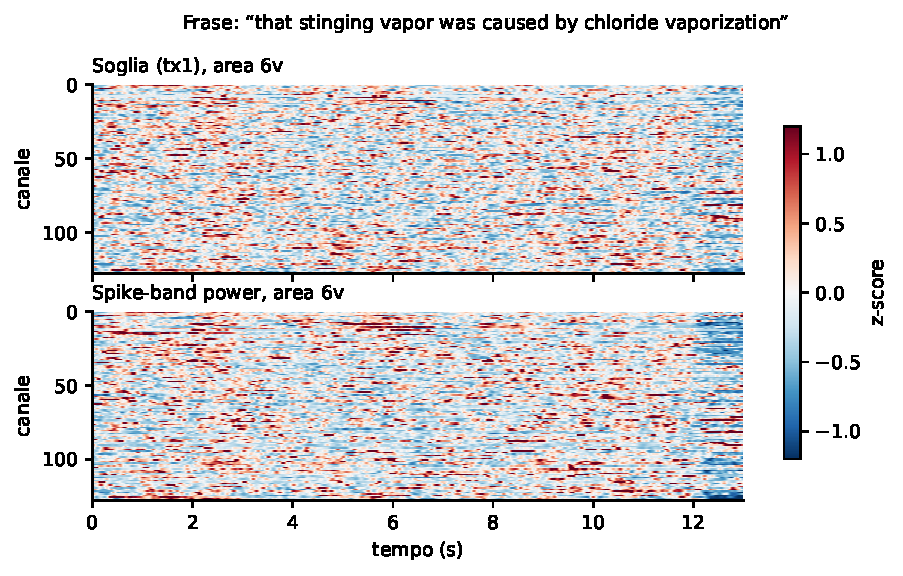
\includegraphics[width=0.92\linewidth]{neural_example.pdf}
\caption{Attività neurale di una frase della partizione di test, normalizzata per blocco e smussata con un filtro gaussiano ($\sigma=40$\,ms). Il segnale è ad alta dimensionalità e molto rumoroso: la struttura legata ai singoli fonemi non è leggibile a occhio, e questo spiega perché servono modelli addestrati su migliaia di frasi.}
\label{fig:neural}
\end{figure}

Le 12\,100 frasi sono state registrate in 24 giorni distribuiti su circa quattro mesi. Per ogni giorno, gli organizzatori hanno assegnato i primi due blocchi alla partizione di gara (\emph{competition hold-out}, 1200 frasi su 15 giorni), l'ultimo blocco al \emph{test} (880 frasi, con trascrizione) e il resto al \emph{train} (8800 frasi). La Fig.~\ref{fig:dataset} mostra come si distribuiscono. Le frasi provengono dal corpus conversazionale Switchboard e da testo web, con un vocabolario molto ampio.

\begin{figure}[t]
\centering
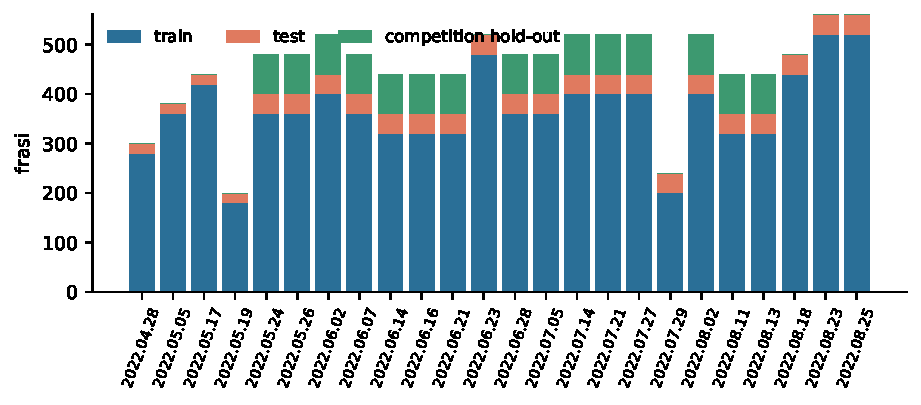
\includegraphics[width=0.92\linewidth]{dataset_days.pdf}\\[2pt]
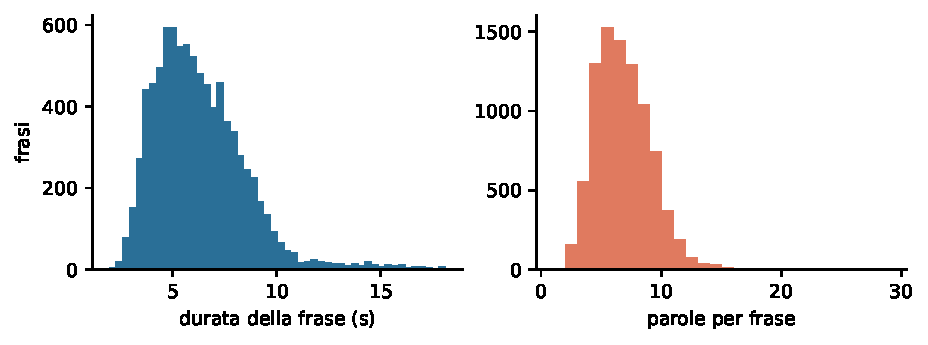
\includegraphics[width=0.92\linewidth]{dataset_hist.pdf}
\caption{In alto: frasi per giorno di registrazione e per partizione. In basso: durata delle frasi del train e numero di parole per frase.}
\label{fig:dataset}
\end{figure}

\paragraph{Non stazionarietà.} Da un giorno all'altro gli elettrodi si spostano di micron, alcuni neuroni smettono di essere registrati e altri compaiono. La stessa intenzione articolatoria produce così pattern di attività diversi in giorni diversi. Il modello deve imparare una rappresentazione comune e insieme una correzione specifica per ogni giorno (Sez.~\ref{sec:model}).

\section{Formulazione}

Il problema ha la stessa struttura del riconoscimento vocale automatico (ASR). Data l'attività $X$, cerchiamo la frase
\begin{equation}
\hat W = \arg\max_W \; p(W\mid X) \;\approx\; \arg\max_W \; \big[\lambda \log p(X\mid W) + \log p(W)\big],
\label{eq:bayes}
\end{equation}
dove $p(X\mid W)$ è un modello ``acustico'' (qui \emph{neurale}) e $p(W)$ un modello del linguaggio. Questa scomposizione è importante con pochi dati: il decoder neurale vede solo 8800 frasi, mentre il modello linguistico può essere addestrato su miliardi di parole di testo.

Come unità intermedia usiamo i \textbf{fonemi}: le 39 classi del dizionario CMU, più un simbolo \texttt{SIL} di fine parola. Le trascrizioni sono convertite in fonemi con il modello \texttt{g2p\_en}. I fonemi sono pochi e condivisi da tutte le parole, quindi il decoder neurale può riconoscere anche parole che non ha mai visto in addestramento.

\paragraph{CTC.} Non sappiamo in quale istante viene pronunciato ciascun fonema, cioè manca l'allineamento fra $X$ e la sequenza fonemica $y$. Usiamo quindi la \emph{Connectionist Temporal Classification} (Graves et al., 2006). Il modello produce per ogni frame $t$ una distribuzione $p_t(k)$ su $K=41$ classi (40 fonemi più un simbolo \emph{blank}). La probabilità di $y$ è la somma su tutti gli allineamenti $\pi$ che, togliendo le ripetizioni e i blank (la funzione $\mathcal{B}$), danno $y$:
\begin{equation}
p_{\text{CTC}}(y\mid X) = \sum_{\pi\in\mathcal{B}^{-1}(y)} \prod_{t=1}^{T'} p_t(\pi_t),
\qquad \mathcal{L} = -\log p_{\text{CTC}}(y\mid X).
\end{equation}
La somma si calcola in tempo $O(T'|y|)$ con un algoritmo forward-backward. La Fig.~\ref{fig:ctc} mostra le distribuzioni $p_t$ prodotte dal nostro modello: picchi stretti sui fonemi, separati da lunghi tratti di blank.

\begin{figure}[t]
\centering
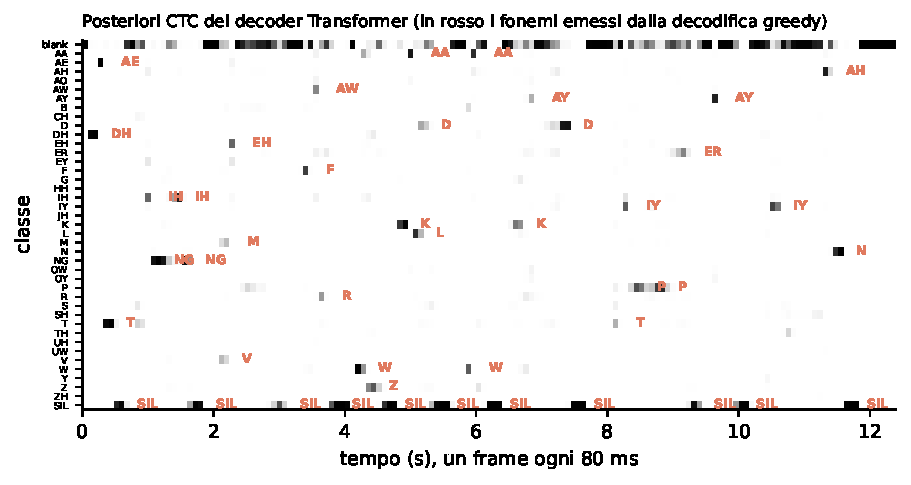
\includegraphics[width=0.95\linewidth]{ctc_posteriors.pdf}
\caption{Probabilità a posteriori delle 41 classi CTC nel tempo, per la frase della Fig.~\ref{fig:neural} (\emph{``that stinging vapor was caused by chloride vaporization''}), dal checkpoint intermedio del Transformer (passo 2500 di 20\,000). In rosso i fonemi scelti dalla decodifica greedy, cioè la classe più probabile in ogni frame, togliendo blank e ripetizioni.}
\label{fig:ctc}
\end{figure}

\section{Il decoder neurale}
\label{sec:model}

L'architettura (Fig.~\ref{fig:pipeline}, blocchi 1--3) riprende la baseline PyTorch degli organizzatori, con le modifiche che il report della gara 2024 indica come utili.

\begin{enumerate}\setlength\itemsep{2pt}
\item \textbf{Smussamento temporale}: convoluzione gaussiana con $\sigma = 2$ bin (40\,ms), per ridurre il rumore di conteggio.
\item \textbf{Strato specifico per giorno}: una trasformazione affine $\tilde x_t = \mathrm{softsign}(W_d x_t + b_d)$, con $W_d\in\mathbb{R}^{256\times256}$ inizializzata all'identità, una per ciascuno dei 24 giorni $d$. Assorbe la deriva fra sessioni e lascia condivisa la parte successiva della rete.
\item \textbf{Finestre temporali}: si concatenano 32 bin consecutivi (640\,ms) con passo 4 (80\,ms). Ogni frame del modello vede un contesto di 0{,}64\,s e la sequenza si accorcia di 4 volte, il che rende più facile il lavoro alla CTC.
\item \textbf{Backbone}, in una di due varianti:
  \begin{itemize}\setlength\itemsep{0pt}
  \item \emph{GRU} bidirezionale, 5 strati da 1024 unità (134\,M parametri), con LayerNorm in ingresso e in uscita;
  \item \emph{Transformer encoder} pre-LN, 5--6 strati con $d=384$--$512$ (13--25\,M parametri), embedding posizionale appreso e attenzione bidirezionale.
  \end{itemize}
\item \textbf{Testa lineare} sulle 41 classi, con log-softmax.
\end{enumerate}

\paragraph{Regolarizzazione e data augmentation.} Con 8800 frasi il sovradattamento è il problema principale. Applichiamo:
\begin{itemize}\setlength\itemsep{0pt}
\item \textbf{rumore gaussiano} sui campioni (\emph{white noise}) e uno spostamento costante per frase e canale (\emph{offset noise}), che simula la deriva dei segnali fra giorni;
\item \textbf{mascheramento temporale}: si azzerano intervalli casuali fino al 30--50\% della frase, una tecnica analoga a SpecAugment che nel lavoro di Feghhi et al.\ (2025) porta il Transformer da 11{,}1\% a 8{,}2\% di WER;
\item \textbf{speckle masking}: si azzerano singoli elementi con probabilità 0{,}3, il che obbliga la rete a non dipendere da singoli canali;
\item \textbf{dropout} di 0{,}2--0{,}4.
\end{itemize}
L'ottimizzazione usa Adam (GRU, con tasso di apprendimento 0{,}02 e decadimento lineare) o AdamW (Transformer, con warm-up e weight decay 0{,}05), in precisione mista fp16 sulle GPU Tesla T4.

\begin{figure}[t]
\centering
\begin{tikzpicture}[
  node distance=4mm and 5mm,
  box/.style={draw, rounded corners=2pt, align=center, font=\footnotesize, minimum height=9mm, text width=24mm, fill=white},
  data/.style={box, fill=bl!10, draw=bl},
  nn/.style={box, fill=or!12, draw=or},
  lm/.style={box, fill=gr!12, draw=gr},
  llm/.style={box, fill=vi!14, draw=vi},
  arr/.style={-{Stealth[length=2mm]}, thick, gray!70!black}
]
\node[data] (x) {Attività neurale\\$X\in\mathbb{R}^{T\times256}$\\(bin 20\,ms)};
\node[nn, right=of x] (pre) {\textbf{1} Smussamento,\\strato per giorno $W_d$,\\softsign};
\node[nn, right=of pre] (win) {\textbf{2} Finestre\\32$\times$20\,ms,\\passo 80\,ms};
\node[nn, right=of win] (bb) {\textbf{3} GRU / Transformer\\+ testa CTC\\$p_t(\text{fonema})$};
\node[lm, below=9mm of bb] (wfst) {\textbf{4} WFST $T\!\circ\! L\!\circ\! G$\\5-gram, beam search\\$\Rightarrow$ 100 frasi};
\node[llm, left=of wfst] (resc) {\textbf{5} Rescoring LLM\\$\lambda s_{ac}+(1\!-\!\alpha)s_{ng}+\alpha s_{llm}$};
\node[llm, left=of resc] (ens) {\textbf{6} Ensemble di $M$\\decoder: fusione con\\LLM addestrato};
\node[data, left=of ens] (out) {Testo\\\emph{``i'm sure there\\are some''}};
\draw[arr] (x) -- (pre); \draw[arr] (pre) -- (win); \draw[arr] (win) -- (bb);
\draw[arr] (bb) -- (wfst); \draw[arr] (wfst) -- (resc); \draw[arr] (resc) -- (ens); \draw[arr] (ens) -- (out);
\begin{scope}[on background layer]
\node[draw=or, dashed, rounded corners, fit=(pre)(bb), inner sep=2.5mm, label={[font=\scriptsize,text=or]above:modello neurale (addestrato con CTC)}] {};
\node[draw=gr!60!vi, dashed, rounded corners, fit=(wfst)(ens), inner sep=2.5mm, label={[font=\scriptsize,text=vi]below:modelli del linguaggio}] {};
\end{scope}
\end{tikzpicture}
\caption{La pipeline completa. Il decoder neurale (blocchi 1--3) trasforma l'attività corticale in probabilità di fonemi. Il trasduttore a stati finiti con il 5-gram (4) produce le frasi candidate, che un LLM riordina (5). Nel passo finale (6) le candidate di molti decoder diversi vengono fuse da un LLM addestrato a correggerle.}
\label{fig:pipeline}
\end{figure}

\section{Dai fonemi alle parole}

\paragraph{Trasduttori a stati finiti.} Il passaggio dalle probabilità di fonemi alle parole usa la composizione di tre trasduttori pesati (WFST), fornita dagli organizzatori e costruita con Kaldi:
\begin{itemize}\setlength\itemsep{0pt}
\item $T$ comprime le sequenze CTC: toglie blank e ripetizioni;
\item $L$ è il lessico: associa a ciascuna delle 125\,000 parole la sua pronuncia in fonemi;
\item $G$ è il modello linguistico 5-gram.
\end{itemize}
Una beam search sul grafo $T\circ L\circ G$ (44\,GB su disco, circa 94\,GB in RAM) trova le frasi che massimizzano l'Eq.~\eqref{eq:bayes}. Sulle CPU del server impiega circa 0{,}3\,s per frase. Per ogni frase conserviamo le 100 ipotesi migliori, ciascuna con il punteggio neurale $s_{ac}$ e quello del 5-gram $s_{ng}$. A ogni frame si sottrae dal blank una penalità $\log 7$, per evitare che il decoder cancelli parole.

Gli organizzatori forniscono anche una versione non potata del 5-gram per un secondo passaggio di rescoring. Richiederebbe circa 300\,GB di RAM, che il server condivide con altri processi: per ora non la usiamo e affidiamo all'LLM il compito di riordinare le ipotesi.

\paragraph{Rescoring con LLM.} Un 5-gram vede solo le quattro parole precedenti. Un LLM invece valuta la frase nella sua interezza: sintassi, semantica, plausibilità. Per ogni ipotesi $h$ calcoliamo $s_{llm}(h)=\sum_j \log p_{\text{LLM}}(h_j\mid h_{<j})$ con OPT-6.7B quantizzato a 8 bit su una T4, e scegliamo
\begin{equation}
\hat h = \arg\max_h \;\big[\lambda\, s_{ac}(h) + (1-\alpha)\, s_{ng}(h) + \alpha\, s_{llm}(h)\big],
\end{equation}
con $\lambda$ e $\alpha$ tarati sulla partizione di test. Sulla CPU l'LLM impiegherebbe circa un secondo per ipotesi, cioè oltre 50 ore per ogni modello: per questo il rescoring gira su GPU.

\section{Ensemble e fusione con LLM}

Secondo il report degli organizzatori sulla gara 2024, il miglioramento più grande è venuto dal combinare molti decoder. Il vincitore (DCoND-LIFT) è passato da 8{,}1\% a 5{,}8\% di WER dando a un LLM addestrato le dieci frasi candidate di dieci modelli diversi, insieme alle relative sequenze di fonemi, e chiedendogli di scrivere la frase corretta. Il sistema impara così che tipo di errori fanno i decoder neurali: fonemi simili scambiati, parole spezzate, omofoni.

Il nostro piano:
\begin{enumerate}\setlength\itemsep{1pt}
\item \textbf{Diversità.} Addestrare decine di decoder che differiscono per architettura, feature, augmentation e seed. Ogni decoder occupa meno di 8\,GB di memoria GPU, quindi le due T4 ne addestrano quattro alla volta.
\item \textbf{Candidate fuori fold.} Per addestrare il fusore servono frasi candidate con errori realistici anche sul train. Lo dividiamo quindi in 5 fold per blocco di registrazione: ogni modello viene addestrato su 4 fold e decodifica il quinto, che non ha visto.
\item \textbf{Fusore.} Addestrare un LLM open-weight da circa 8 miliardi di parametri con QLoRA (pesi a 4 bit più adattatori a basso rango), che entra in una T4 da 16\,GB. Riceve le $M$ candidate e restituisce la trascrizione.
\item \textbf{Combinazione finale.} Votazione (ROVER) fra le uscite di più fusori, e in alternativa un LLM generalista recente usato senza addestramento, con esempi nel prompt.
\end{enumerate}

\section{Primi risultati}

La Fig.~\ref{fig:curves} mostra il \emph{phoneme error rate} (PER) sul test durante l'addestramento, misurato con la decodifica greedy, cioè senza modello linguistico. I Transformer con mascheramento temporale convergono più rapidamente del GRU: dopo 5000 passi su 20\,000 sono già intorno al 22\% di PER.

\begin{figure}[t]
\centering
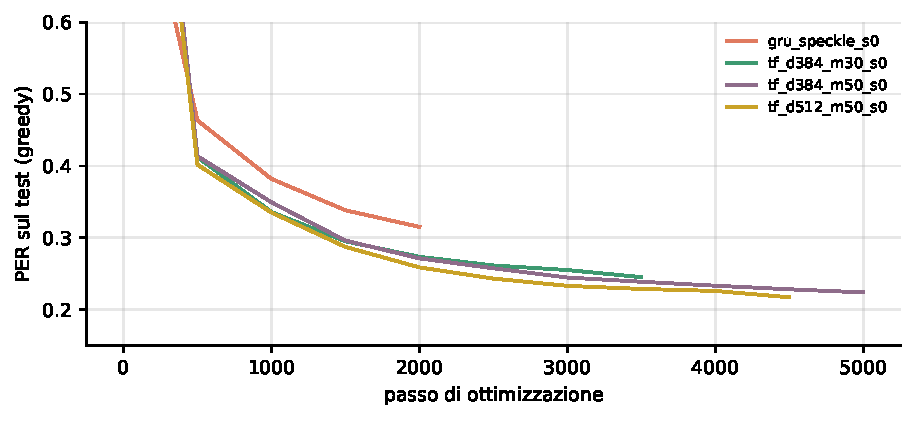
\includegraphics[width=0.9\linewidth]{training_curves.pdf}
\caption{PER sul test durante l'addestramento dei primi quattro decoder, in corso al momento della stesura. \texttt{tf\_d384\_m50}: Transformer con $d=384$ e il 50\% del tempo mascherato. \texttt{gru\_speckle}: GRU bidirezionale con speckle masking. Per costruzione il GRU è più lento per passo.}
\label{fig:curves}
\end{figure}


\paragraph{Prima decodifica completa.} Per verificare la pipeline da un capo all'altro abbiamo esportato un checkpoint intermedio del Transformer (\texttt{tf\_d384\_m50} al passo 2500, PER greedy 25{,}8\%) e lo abbiamo decodificato con il 5-gram. Sul test il WER 1-best è del \textbf{25{,}9\%}, ancora senza rescoring LLM, con i parametri di decodifica della baseline ($\lambda=0{,}5$, penalità di blank $\log 7$) e con un modello fermo al passo 2500 di 20\,000. Non è un risultato competitivo: serve a confermare che tutti i componenti funzionano insieme. La Tab.~\ref{tab:esempi} mostra alcune frasi decodificate.

Dagli esempi si vede come lavora il modello linguistico. Per la frase \emph{``i'm sure there are some''} la decodifica greedy produce i fonemi
\begin{center}\small\texttt{AY M | SH UH R | DH EH R | AW R | T AY M |}\end{center}
(\texttt{|} indica la fine di una parola). La sequenza contiene errori (\texttt{AW R} per \emph{are}, \texttt{T AY M} per \emph{some}), ma il 5-gram li corregge e restituisce la frase esatta. Quando invece gli errori fonetici sono molti, il 5-gram sceglie una frase plausibile in inglese ma sbagliata (\emph{``spinal tap''} per \emph{``financial type''}): è proprio il caso in cui contano un decoder neurale migliore, un LLM che guardi tutta la frase e l'ensemble.

\begin{table}[h]
\centering\small
\begin{tabularx}{\linewidth}{>{\raggedright\arraybackslash}X >{\raggedright\arraybackslash}X c}
\toprule
\textbf{Frase pronunciata (riferimento)} & \textbf{Decodifica neurale + 5-gram} & \\
\midrule
\textit{that stinging vapor was caused by chloride vaporization} & that thing as it was called was called up in &  \\
\textit{a sharp tremor was followed by a jerky roll} & a top team with killed by a truck while &  \\
\textit{that's a science in itself} & that's a science in itself & \checkmark \\
\textit{i'm sure there are some} & i'm sure there are some & \checkmark \\
\textit{most people aren't} & more people want &  \\
\textit{it's a little bit financial type thing} & it's a little bit spinal tap thing &  \\
\bottomrule
\end{tabularx}
\caption{Esempi reali dalla partizione di test, decodificati dal checkpoint intermedio con il 5-gram (ipotesi migliore su 100), senza rescoring LLM.}
\label{tab:esempi}
\end{table}

\begin{table}[h]
\centering\small
\begin{tabular}{lcc}
\toprule
\textbf{Sistema} & \textbf{WER} & \textbf{Fonte} \\
\midrule
Baseline NPTL: RNN + 5-gram + OPT & 9{,}76\% & classifica EvalAI \\
DCoND-LIFT, vincitore 2024 (ensemble + GPT-3.5 addestrato) & 5{,}77\% & classifica, arXiv:2411.10657 \\
Miglior metodo pubblicato (LightBeam) & 4{,}98\% & classifica, arXiv:2603.14002 \\
Primo classificato (metodo non pubblicato) & 2{,}99\% & classifica, 22/11/2026 \\
\midrule
Questo lavoro: checkpoint intermedio + 5-gram (sul test) & 25{,}9\% & questo documento \\
\bottomrule
\end{tabular}
\caption{Contesto: i numeri della classifica sono misurati sulla partizione di gara, il nostro sul test. I due valori non sono direttamente confrontabili.}
\label{tab:classifica}
\end{table}


\section{Infrastruttura}

\begin{itemize}\setlength\itemsep{0pt}
\item \textbf{Server:} un server di ateneo con 64 thread CPU, 372\,GB di RAM e due NVIDIA Tesla T4 da 16\,GB.
\item \textbf{Esecuzione:} tutto gira in sessioni \texttt{screen} indipendenti.
\item \textbf{Addestramento:} una coda di job su file alimenta quattro worker, due per GPU. Se un job va in out-of-memory viene rimesso in coda.
\item \textbf{Decodifica:} un servizio carica il 5-gram una sola volta e decodifica automaticamente ogni nuovo modello.
\item \textbf{Orchestrazione:} un orchestratore accoda il rescoring LLM e produce il file di sottomissione.
\item \textbf{Vincoli:} il driver CUDA 12.2 impone PyTorch 2.7, e il decoder WFST (C++, WeNet e Kaldi) usa un ambiente Python separato con libtorch 1.13.
\end{itemize}

\section{Limiti e prossimi passi}

\begin{itemize}\setlength\itemsep{1pt}
\item \textbf{Validazione.} Il test (880 frasi) serve sia a scegliere gli iperparametri sia a stimare il WER, quindi la stima è ottimista. Le sottomissioni a EvalAI (cinque al giorno) sono l'unica misura imparziale.
\item \textbf{Metodi dei primi classificati.} I primi tre non hanno pubblicato il metodo. Il miglior risultato con metodo pubblicato è 4{,}98\%: scendere sotto il 3\% richiede di andare oltre lo stato dell'arte pubblicato.
\item \textbf{Sviluppi possibili:}
  \begin{itemize}\setlength\itemsep{0pt}
  \item target a difoni (DCoND);
  \item pre-addestramento su altri dataset pubblici di speech BCI, per esempio il partecipante T15 della gara 2025;
  \item adattamento non supervisionato sui giorni della partizione di gara (\emph{test-time adaptation});
  \item un LLM di fusione più grande.
  \end{itemize}
\end{itemize}

\paragraph{Riferimenti principali.}
\begin{itemize}\setlength\itemsep{0pt}
\item F.\,R.\ Willett et al., \emph{A high-performance speech neuroprosthesis}, Nature 620 (2023).
\item F.\,R.\ Willett et al., \emph{Brain-to-Text Benchmark '24: lessons learned}, arXiv:2412.17227.
\item A.\ Graves et al., \emph{Connectionist Temporal Classification}, ICML 2006.
\item J.\ Li et al., \emph{DCoND-LIFT}, arXiv:2411.10657.
\item E.\ Feghhi et al., \emph{Time-masked Transformers for speech BCI}, arXiv:2507.02800.
\end{itemize}

\end{document}
